%!TEX root = ./RfCPN.tex


\addtocontents{toc}{\protect\cleardoublepage}
%%%%%%%%%%%%%%%%%%%%%%%%%%%%%%%%%%%%%%%%%%%%%%%%%%%%%%%%%
%% Part Requirement Definition %%%%%%%%%%%%%%%%%%%%%%%%%%
%%%%%%%%%%%%%%%%%%%%%%%%%%%%%%%%%%%%%%%%%%%%%%%%%%%%%%%%%
\addtocontents{toc}{\protect\begin{tocBox}{\tmppartnum}}%
\tPart[lof]{加工システムの設計\TBW}{%
\paragraph*{\tpartgoal}
加工システムの作成に向けて、その設計を行う。

\tcbline*
\paragraph*{\tpartmethod}
策定した諸標準や解析的・数値的導出した幾何的情報を用いて、抽出した\index{ようけん@要件}要件を満たすよう設計を行う。

\tcbline*
\paragraph*{\tpartbackground}
(to be written...)
}{%
\paragraph*{\tpartconclusion}
(to be written...)
\tcbline*
\paragraph*{\tpartnextstep}
設計にしたがって、具体的な\index{NCプログラム}NCプログラムの作成を行う。
}

%%%%%%%%%%%%%%%%%%%%%%%%%%%%%%%%%%%%%%%%%%%%%%%%%%%%%%%%%
%% chapters %%%%%%%%%%%%%%%%%%%%%%%%%%%%%%%%%%%%%%%%%%%%%
%%%%%%%%%%%%%%%%%%%%%%%%%%%%%%%%%%%%%%%%%%%%%%%%%%%%%%%%%
%!TEX root = ../RfCPN.tex


\modHeadchapter[lof]{加工システムの全体の流れと必要なNCサブプログラム}
%%%%%%%%%%%%%%%%%%%%%%%%%%%%%%%%%%%%%%%%%%%%%%%%%%%%%%%%%%
%% figure %%%%%%%%%%%%%%%%%%%%%%%%%%%%%%%%%%%%%%%%%%%%%%%%
%%%%%%%%%%%%%%%%%%%%%%%%%%%%%%%%%%%%%%%%%%%%%%%%%%%%%%%%%%
\begin{figure}[p]%
\begin{Figlandscape}
\begin{adjustbox}{%
  addcode={\begin{minipage}{\textheight}\centering}{%
    \captionof{figure}{加工全体のフロー(概要)\label{fig:flowchart}}%
    \end{minipage}%
  },
  rotate=90,
  center,
%  max width=\textheight,
%  max height=\linewidth,
  keepaspectratio}
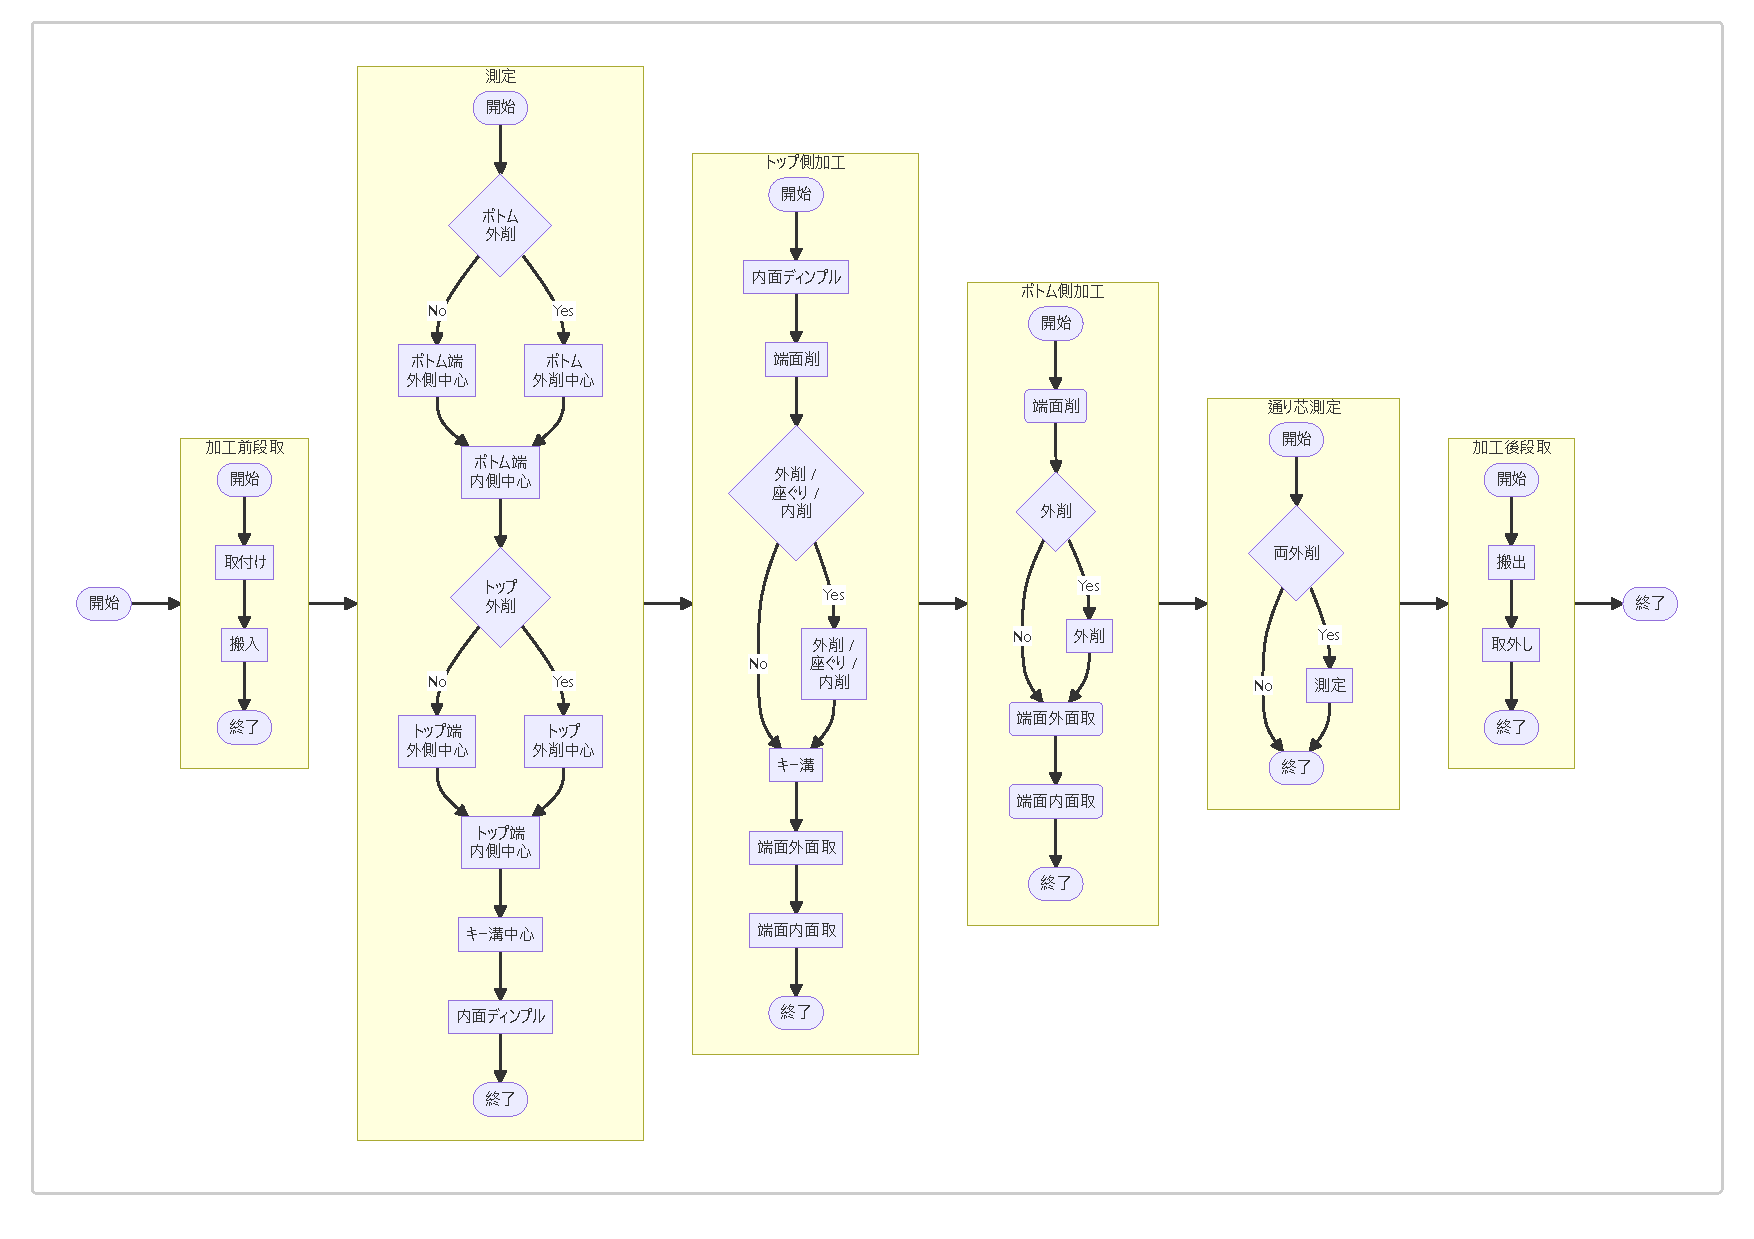
\includegraphics[height=\linewidth-10pt, trim=20 30 20 20, clip]{RfCPN_p03_pictures/Milling_flow_chart.pdf}%
\end{adjustbox}
\end{Figlandscape}%
\end{figure}%
%%%%%%%%%%%%%%%%%%%%%%%%%%%%%%%%%%%%%%%%%%%%%%%%%%%%%%%%%%
%%%%%%%%%%%%%%%%%%%%%%%%%%%%%%%%%%%%%%%%%%%%%%%%%%%%%%%%%%
%%%%%%%%%%%%%%%%%%%%%%%%%%%%%%%%%%%%%%%%%%%%%%%%%%%%%%%%%%



%%%%%%%%%%%%%%%%%%%%%%%%%%%%%%%%%%%%%%%%%%%%%%%%%%%%%%%%%%
%% section 06.01 %%%%%%%%%%%%%%%%%%%%%%%%%%%%%%%%%%%%%%%%%
%%%%%%%%%%%%%%%%%%%%%%%%%%%%%%%%%%%%%%%%%%%%%%%%%%%%%%%%%%
\modHeadsection{加工全体の流れ}
加工全体の流れは\pageautoref{sec:MillingSystemFlow}に基づく。


%%%%%%%%%%%%%%%%%%%%%%%%%%%%%%%%%%%%%%%%%%%%%%%%%%%%%%%%%%
%% subsection 06.02.01 %%%%%%%%%%%%%%%%%%%%%%%%%%%%%%%%%%%
%%%%%%%%%%%%%%%%%%%%%%%%%%%%%%%%%%%%%%%%%%%%%%%%%%%%%%%%%%
\subsection{工程:加工前の段取}
\begin{enumerate}[label*=\sarrow]
\item ワークを\Table 上の\Jig に取り付ける
\item \Palette を交換し、ワークを機内に搬入する
\end{enumerate}


%%%%%%%%%%%%%%%%%%%%%%%%%%%%%%%%%%%%%%%%%%%%%%%%%%%%%%%%%%
%% subsection 06.02.02 %%%%%%%%%%%%%%%%%%%%%%%%%%%%%%%%%%%
%%%%%%%%%%%%%%%%%%%%%%%%%%%%%%%%%%%%%%%%%%%%%%%%%%%%%%%%%%
\subsection{工程:加工前の測定}

%%%%%%%%%%%%%%%%%%%%%%%%%%%%%%%%%%%%%%%%%%%%%%%%%%%%%%%%%%
%% subsubsection 06.02.02.1 %%%%%%%%%%%%%%%%%%%%%%%%%%%%%%
%%%%%%%%%%%%%%%%%%%%%%%%%%%%%%%%%%%%%%%%%%%%%%%%%%%%%%%%%%
\subsubsection{ワーク座標系原点設定}
\begin{enumerate}[label*=\sarrow]
\item ボトム側が工具側になるよう回転する
\item \BottomEndFace 部の外側中心を測定する
\item \BottomEndFace 部の内側中心を測定する
\item トップ側が工具側になるよう回転する
\item \TopEndFace 部の外側中心を測定する
\item \TopEndFace 部の内側中心を測定する
\item \KeywayCenter を測定する
\end{enumerate}

%%%%%%%%%%%%%%%%%%%%%%%%%%%%%%%%%%%%%%%%%%%%%%%%%%%%%%%%%%
%% subsubsection 06.02.02.1 %%%%%%%%%%%%%%%%%%%%%%%%%%%%%%
%%%%%%%%%%%%%%%%%%%%%%%%%%%%%%%%%%%%%%%%%%%%%%%%%%%%%%%%%%
\subsubsection{\DimpleMeasurement}
\begin{enumerate}[label*=\sarrow]
\item すべての\Dimple の表面位置を測定する
\end{enumerate}


%%%%%%%%%%%%%%%%%%%%%%%%%%%%%%%%%%%%%%%%%%%%%%%%%%%%%%%%%%
%% subsection 06.02.03 %%%%%%%%%%%%%%%%%%%%%%%%%%%%%%%%%%%
%%%%%%%%%%%%%%%%%%%%%%%%%%%%%%%%%%%%%%%%%%%%%%%%%%%%%%%%%%
\subsection{工程:トップ側の加工}
\begin{enumerate}[label*=\sarrow]
\item \DimpleMilling を行う
\item \TopEndFacecutMilling を行う
\item (存在する場合)\TopOutcutMilling を行う
\item (存在する場合)\TopCurvedOutcutMilling を行う
\item (存在する場合)\EndFaceBoringMilling を行う
\item (存在する場合)\IncutBoringMilling を行う
\item \TopEndFaceOutCChamferMilling を行う
\item \TopEndFaceInCChamferMilling を行う
\end{enumerate}


\clearpage
%%%%%%%%%%%%%%%%%%%%%%%%%%%%%%%%%%%%%%%%%%%%%%%%%%%%%%%%%%
%% subsection 06.02.04 %%%%%%%%%%%%%%%%%%%%%%%%%%%%%%%%%%%
%%%%%%%%%%%%%%%%%%%%%%%%%%%%%%%%%%%%%%%%%%%%%%%%%%%%%%%%%%
\subsection{工程:ボトム側の加工}
\begin{enumerate}[label*=\sarrow]
\item ボトム側が工具側になるよう回転する
\item \BottomEndFacecutMilling を行う
\item (存在する場合)\BottomOutcutMilling を行う
\item (存在する場合)\BottomCurvedOutcutMilling を行う
\item \BottomEndFaceOutCChamferMilling を行う
\item \BottomEndFaceInCChamferMilling を行う
\end{enumerate}


%%%%%%%%%%%%%%%%%%%%%%%%%%%%%%%%%%%%%%%%%%%%%%%%%%%%%%%%%%
%% subsection 06.02.05 %%%%%%%%%%%%%%%%%%%%%%%%%%%%%%%%%%%
%%%%%%%%%%%%%%%%%%%%%%%%%%%%%%%%%%%%%%%%%%%%%%%%%%%%%%%%%%
\subsection{工程:加工後の測定}
\begin{enumerate}[label*=\sarrow]
\item \TopOutcut と\BottomOutcut の両方が存在する場合、\CenterlineEndFaceDifMeasurement を行う
\end{enumerate}


%%%%%%%%%%%%%%%%%%%%%%%%%%%%%%%%%%%%%%%%%%%%%%%%%%%%%%%%%%
%% subsection 41.01.06 %%%%%%%%%%%%%%%%%%%%%%%%%%%%%%%%%%%
%%%%%%%%%%%%%%%%%%%%%%%%%%%%%%%%%%%%%%%%%%%%%%%%%%%%%%%%%%
\subsection{工程:加工後の段取}
\begin{enumerate}[label*=\sarrow]
\item \Palette を交換し、ワークを機外に搬出する
\item ワークを\Table 上の\Jig から取り外す41
\end{enumerate}



\clearpage
%%%%%%%%%%%%%%%%%%%%%%%%%%%%%%%%%%%%%%%%%%%%%%%%%%%%%%%%%%
%% section 41.02 %%%%%%%%%%%%%%%%%%%%%%%%%%%%%%%%%%%%%%%%%
%%%%%%%%%%%%%%%%%%%%%%%%%%%%%%%%%%%%%%%%%%%%%%%%%%%%%%%%%%
\modHeadsection{必要なNCサブプログラム\TBW}
(to be written...)




%%%%%%%%%%%%%%%%%%%%%%%%%%%%%%%%%%%%%%%%%%%%%%%%%%%%%%%%%
%% Appendices %%%%%%%%%%%%%%%%%%%%%%%%%%%%%%%%%%%%%%%%%%%
%%%%%%%%%%%%%%%%%%%%%%%%%%%%%%%%%%%%%%%%%%%%%%%%%%%%%%%%%
\begin{appendices}
%\Appendixpart
\end{appendices}

\addtocontents{toc}{\protect\end{tocBox}}
